% !TEX program = xelatex
\documentclass[11pt, aspectratio=169]{beamer}
\usetheme{metropolis}
\useoutertheme{metropolis}
\useinnertheme{metropolis}
\usecolortheme{metropolis}
\usefonttheme{professionalfonts} % [Beamer 설정] Beamer가 폰트를 건드리지 못하게 함 (필수)

\usepackage{kotex}
\usepackage{tikz} 
\usepackage{graphicx, caption, hyperref, fontawesome5}

% [수식 및 폰트 핵심 설정]
\usepackage{amsmath}
\usepackage[math-style=ISO, bold-style=ISO]{unicode-math} % unicode-math 로드

% 1. Beamer가 폰트를 제멋대로 바꾸지 못하게 막음 (필수!)
\usefonttheme{professionalfonts}

% 2. 본문 폰트 설정 (Pretendard)
% AutoFakeSlant: 이탤릭체가 없는 Pretendard를 위해 강제로 20% 기울임
\setmainfont[Ligatures=TeX, BoldFont={* Bold}, AutoFakeSlant=0.2]{Pretendard}
\setsansfont[Ligatures=TeX, BoldFont={* Bold}, AutoFakeSlant=0.2]{Pretendard}
\setmainhangulfont[BoldFont={* Bold}]{Pretendard}
\setsanshangulfont[BoldFont={* Bold}]{Pretendard}

% 3. 수식 폰트 설정 (Fira Math + Pretendard 조합)
% (A) 기본 수식 기호는 Fira Math (Sans-serif Math Font) 사용
\setmathfont{Fira Math}

% (B) 수식 내의 문자(x, y, log, sin 등)는 Pretendard로 덮어씌움 (통일감)
\setmathfont[range={up, bfup}, Scale=MatchLowercase]{Pretendard}
\setmathfont[range={it, bfit}, Scale=MatchLowercase, FakeSlant=0.2]{Pretendard}

% 4. 메타데이터
\title{Communication Theory - 2026}
\subtitle{CDMA 시스템과 Viterbi 복호화}
\date{\today}
\author{
    이 경 근 \\
    {\tiny
        \raisebox{0.1ex}{\scalebox{0.85}{\faEnvelope}} \href{mailto:infosec@knu.ac.kr}{infosec@knu.ac.kr} \quad 
        {\scalebox{0.9}{\faLinkedin}} \scalebox{0.9}{\href{https://www.linkedin.com/in/Kenny-0633-Lee}{Kenny-0633-Lee}}
    }
}
\institute{EE / KNU}
\graphicspath{{./assets/}}


%%%%%%%%%%%%%%%%%%%%%%%%%%%%%%%%%%%%%%%%%%%%%
%%%%%%%%%%%%%%%%%%%%%%%%%%%%%%%%%%%%%%%%%%%%%

\begin{document}

% Title Page
\begin{frame}[plain]
    \titlepage
\end{frame}

\begin{frame}
    \[
        \int_0^{\pi} \sin x \, \mathrm{d}x = 2
    \]

\end{frame}

% --- Introduction ---
\begin{frame}{Introduction}
    \centering
    Python과 LaTeX의 완벽한 분리(Decoupling)를 통한\\
    \textbf{안정적인 강의 자료 시스템}입니다.
\end{frame}

% --- 강의 범위 및 시각화 계획 (Lathi Ch 1-7) ---
\begin{frame}{강의 범위 및 시각화 계획 (Lathi Ch 1-7)}
    \begin{itemize}
        \item \textbf{Ch 1-3:} 신호와 시스템 (Time/Freq Plot)
        \item \textbf{Ch 4-5:} 아날로그 변조 (AM/FM Waveform)
        \item \textbf{Ch 6-7:} 디지털 통신 (Sampling, Constellation)
    \end{itemize}
\end{frame}

% ... (이전 "강의 범위 및 시각화 계획" 프레임 끝) ...

% --- [NEW] Ch 01. Shannon Theory ---
\begin{frame}{Chapter 01. Why Bandwidth is Revenue}
    \begin{columns}
        % [Left] Python Generated Visual
        \begin{column}{0.6\textwidth}
            \centering
            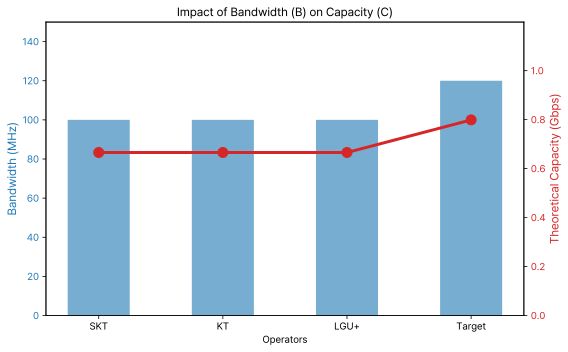
\includegraphics[width=\textwidth]{fig_ch01_shannon.pdf}
        \end{column}
        
        % [Right] Mathematical Proof
        \begin{column}{0.4\textwidth}
            \begin{block}{Shannon-Hartley Theorem}
                \centering
                $C = \mathbf{B} \log_2 \left( 1 + \frac{S}{N} \right)$
            \end{block}
            
            \vspace{0.3cm}
            \textbf{Key Insight:}
            \begin{itemize}
                \item \textbf{Bandwidth ($\mathbf{B}$):} \\
                Capacity와 \textcolor{red}{선형(Linear)} 비례 \\
                $\rightarrow$ \textit{"돈으로 대역폭을 사는 이유"}
                
                \item \textbf{Power ($S$):} \\
                Capacity와 \textcolor{blue}{로그(Log)} 비례 \\
                $\rightarrow$ \textit{"효율 체감의 법칙"}
            \end{itemize}
        \end{column}
    \end{columns}
\end{frame}

% --- Ch 3. Channel 예제 ---
\begin{frame}{Practical Application: 5G Spectrum in Korea}
    \centering
    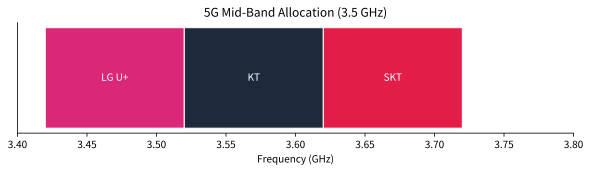
\includegraphics[width=0.9\textwidth]{fig_ch3_5g_spectrum.pdf}
    
    \vspace{0.5cm}
    \begin{block}{Shannon-Hartley Theorem in Practice}
        $C = \mathbf{B} \log_2(1 + SNR)$
        \begin{itemize}
            \item \textbf{mmWave (28GHz):} $B = 800\text{MHz}$ $\rightarrow$ Ultra-high Capacity
            \item \textbf{Sub-6 (3.5GHz):} $B = 100\text{MHz}$ $\rightarrow$ National Coverage
        \end{itemize}
    \end{block}
    \small \textit{Observation: 광대역 연속 블록 확보가 스펙트럼 효율의 핵심입니다.}
\end{frame}

% --- Ch 4. AM 예제 ---
\begin{frame}{Chapter 4. Amplitude Modulation}
    \begin{columns}
        \begin{column}{0.5\textwidth}
            \textbf{Time Domain}
            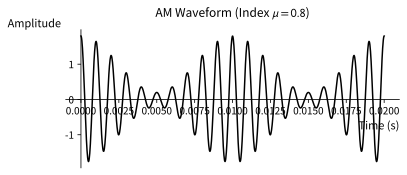
\includegraphics[width=\textwidth]{fig_ch4_am_time.pdf}
        \end{column}
        \begin{column}{0.5\textwidth}
            \textbf{Frequency Domain}
            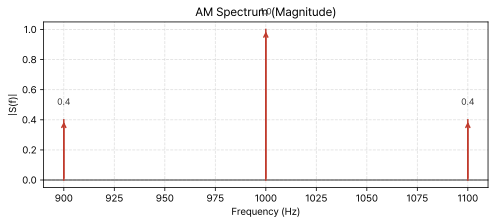
\includegraphics[width=\textwidth]{fig_ch4_am_spec.pdf}
        \end{column}
    \end{columns}
    \vspace{0.2cm}
    \centering
    \small AM 신호는 시간 영역의 포락선(Envelope)과 주파수 영역의 측파대(Sidebands)로 해석됩니다.
\end{frame}

% --- Ch 7. Digital 예제 ---
\begin{frame}{Chapter 7. Digital Modulation (QPSK)}
    \begin{columns}
        \begin{column}{0.6\textwidth}
            \centering
            % 정사각형 비율 유지를 위해 height 지정
            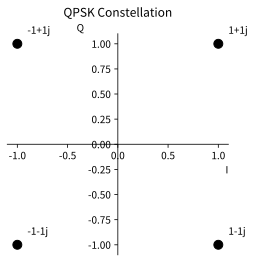
\includegraphics[height=0.6\textheight]{fig_ch7_qpsk.pdf}
        \end{column}
        \begin{column}{0.4\textwidth}
            \textbf{QPSK 특징:}
            \begin{itemize}
                \item 2 bits per symbol
                \item 4개의 위상 상태
                \item 대역폭 효율성 증대
            \end{itemize}
        \end{column}
    \end{columns}
\end{frame}


% --- Closing ---
\begin{frame}{강의 Recap.}
    \centering
    \begin{itemize}
        \item Python을 통한 신호 생성 및 시각화
        \item LaTeX Beamer로 안정적인 프레젠테이션 제작
        \item $C = \mathbf{B} \log_2 \left( 1 + \frac{S}{N} \right)$
        \item 통신 이론의 핵심 개념들을 시각적으로 이해
    \end{itemize}
\end{frame}

\end{document}